% =============================================================================
%  P2 - Segmentação temporal no sistema de Gray-Scott (The Well)
%  Processamento de Imagens - UFMA
%
%  14 slides para 12 minutos (cerca de 50 s por slide).
%  Mesmo tema e paleta da apresentação do T1.
%
%  Compilar com XeLaTeX:  latexmk -xelatex apresentacao.tex
% =============================================================================

\documentclass[aspectratio=169,11pt]{beamer}

\newcommand{\autores}{ANDRE LUIS AGUIAR DO NASCIMENTO \\
JOAO GUILHERME MIRANDA LAGO \\
WESLEY DOS SANTOS GATINHO}
\newcommand{\professor}{Prof. HAROLDO GOMES BARROSO FILHO}

\usetheme[progressbar=none, numbering=fraction, block=fill, sectionpage=none]{metropolis}

\usepackage{fontspec}
\setsansfont{Fira Sans}[Numbers=Lining]
\setmonofont{Fira Mono}[Scale=0.82]
\usepackage[brazil]{babel}
\usepackage{amsmath, amssymb}
\usepackage{booktabs}
\usepackage{array}
\usepackage{graphicx}
\usepackage{tikz}
\usetikzlibrary{positioning,arrows.meta,calc,babel}

\graphicspath{{figuras/}}

\definecolor{ink}{HTML}{16262E}
\definecolor{cinza}{HTML}{5A6B73}
\definecolor{papel}{HTML}{FAFAF8}
\definecolor{marca}{HTML}{9A3B26}

\setbeamercolor{normal text}{fg=ink, bg=papel}
\setbeamercolor{alerted text}{fg=marca}
\setbeamercolor{frametitle}{bg=ink, fg=papel}
\setbeamercolor{title separator}{fg=marca}
\setbeamerfont{frametitle}{size=\large}
\setbeamertemplate{itemize items}[circle]
\setlength{\parskip}{.35em}

\newcommand{\leg}[1]{{\small\textcolor{cinza}{#1}}}
\newcommand{\ind}{\mathbf{1}}

\title{Segmentação temporal no sistema de Gray-Scott}
\subtitle{Pré-processamento, arquiteturas e pós-processamento}
\author{\autores}
\institute{Processamento de Imagens \\ Universidade Federal do Maranhão \\ \professor}
\date{Trabalho P2}

\begin{document}

\maketitle

% =============================================================================
\begin{frame}{Problema}

  Em um campo de concentração que muda no tempo, queremos saber
  \textbf{onde estão as estruturas} e \textbf{como elas evoluem}: quando surgem,
  como se dividem, para onde migram e quando desaparecem.

  Para isso o campo precisa virar regiões, ou seja, ser segmentado a cada instante.

  \vspace{.3em}
  O protocolo da turma fixa o experimento para todos os fluidos:
  \begin{itemize}
    \item 10 pré-processamentos, 3 arquiteturas e 5 pós-processamentos;
    \item entrada de no máximo 128 pixels, sem ampliação, e até 25~GB de dados;
    \item 20 épocas de treino para todas as redes;
    \item quatro condições: só a rede, pré + rede, rede + pós, pré + rede + pós.
  \end{itemize}

\end{frame}

% =============================================================================
\section{O sistema físico}

% -----------------------------------------------------------------------------
\begin{frame}{Modelo de Gray-Scott}

  Um substrato $A$ é consumido pela reação autocatalítica $A+2B\to3B$:

  \vspace{-.6em}
  \begin{align*}
    \partial_t A &= \delta_A\nabla^2 A - AB^2 + F(1-A)\\
    \partial_t B &= \delta_B\nabla^2 B + AB^2 - (F+k)B
  \end{align*}

  \vspace{-.4em}
  \begin{itemize}
    \item $F$ alimenta $A$, $k$ remove $B$. Pequenas mudanças em $(F,k)$ mudam o padrão.
    \item Com $\delta_A=2\delta_B$ surge a instabilidade de Turing: manchas, labirintos, ondas.
    \item Para alguns parâmetros o padrão colapsa e as estruturas somem.
  \end{itemize}

  \leg{Aplicações: reatores químicos (região de ignição), vazamentos de gás
  reativo em segurança industrial, padrões biológicos e diagnóstico de
  modelos substitutos neurais.}

\end{frame}

% -----------------------------------------------------------------------------
\begin{frame}{Os seis regimes do conjunto}

  \begin{columns}[c,onlytextwidth]
    \column{.66\textwidth}
      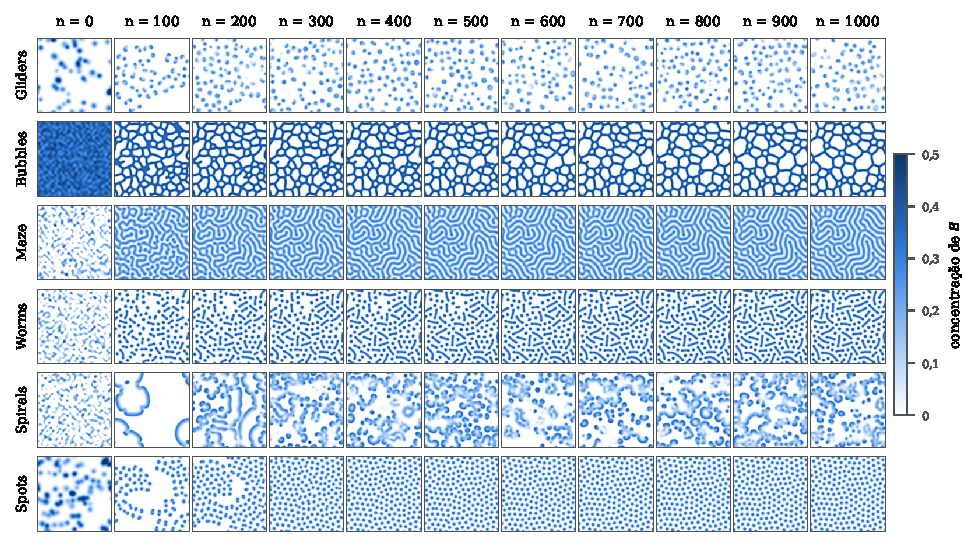
\includegraphics[width=\textwidth]{fluid_by_time}
    \column{.31\textwidth}
      \small
      1.200 trajetórias, 200 por regime.

      Grade periódica de $128\times128$, com 1.001 instantes por trajetória.

      Em $n=0$ a condição inicial é aleatória; o padrão se organiza nos
      primeiros instantes.

      \leg{Concentração de $B$ em uma trajetória de teste por regime.}
  \end{columns}

\end{frame}

% -----------------------------------------------------------------------------
\begin{frame}{Referência de segmentação}

  \begin{columns}[c,onlytextwidth]
    \column{.42\textwidth}
      \small
      Estrutura é a região de reação ativa, onde $B$ é alto:
      \[ M_i(x,y,n)=\ind\,[\,B_i(x,y,n)>\tau_i\,] \]
      $\tau_i$ é o limiar de Otsu de $B$ em $n=500$, fixo para toda a trajetória.

      A rede recebe \textbf{só o campo $A$}. Como $A$ e $B$ são
      anticorrelacionados, Otsu em $A$ serve de referência sem aprendizado.

      \leg{Nas 95 trajetórias já extintas em $n=500$ usou-se a mediana dos
      limiares do regime no treino.}
    \column{.55\textwidth}
      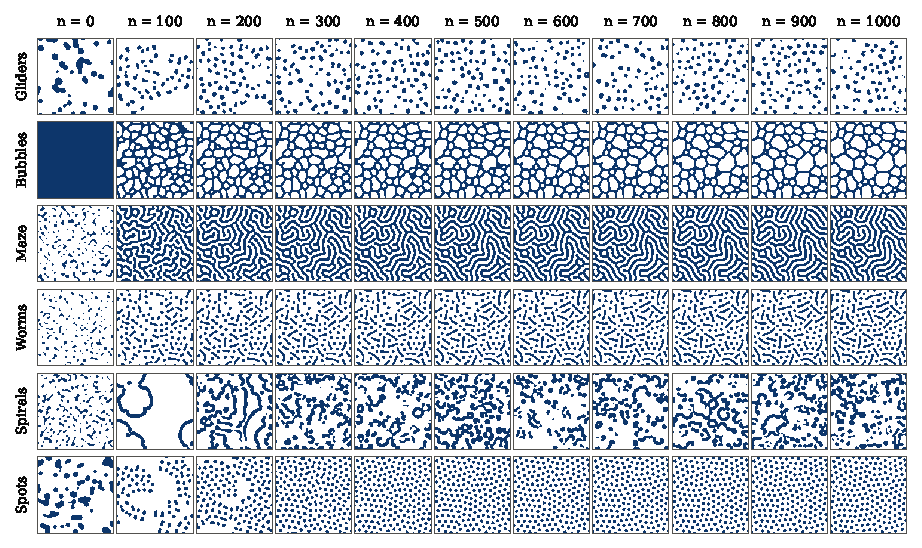
\includegraphics[width=\textwidth]{gt_by_time}
  \end{columns}

\end{frame}

% =============================================================================
\section{Protocolo}

% -----------------------------------------------------------------------------
\begin{frame}{Dados e pipeline}

  \centering
  \resizebox{!}{.6\textheight}{%
  \begin{tikzpicture}[node distance=5mm and 5mm, >=Stealth, font=\footnotesize,
    caixa/.style={draw=cinza, rounded corners=2pt, align=center, minimum height=12mm, inner sep=3pt, fill=white, text width=31mm},
    dados/.style={caixa, fill=gray!8},
    prep/.style={caixa, fill=orange!12},
    rede/.style={caixa, fill=blue!8, text width=24mm, minimum height=7mm},
    posproc/.style={caixa, fill=teal!12},
    aval/.style={caixa, fill=violet!8}]
  \node[dados] (well) {\textbf{The Well}\\ 1.200 trajetórias\\ $1001\times128\times128$};
  \node[dados, right=of well] (sub) {\textbf{Subconjunto}\\ todas as trajetórias\\ 21 instantes, 3,3 GB};
  \node[dados, right=of sub] (res) {\textbf{Resolução nativa}\\ $128\times128$\\ sem reamostragem};
  \node[dados, right=of res] (gt) {\textbf{Referência}\\ Otsu em $B$, $n=500$};
  \node[dados, right=of gt] (part) {\textbf{Partições oficiais}\\ 960 / 120 / 120};
  \draw[->] (well) -- (sub); \draw[->] (sub) -- (res); \draw[->] (res) -- (gt); \draw[->] (gt) -- (part);
  \node[dados, below=16mm of well] (ent) {\textbf{Entrada $A$}};
  \node[prep, right=of ent] (pre) {\textbf{Pré}\\ P0 e P1 a P10};
  \node[rede, right=of pre, yshift=9mm] (u) {U-Net};
  \node[rede, right=of pre] (s) {SegFormer};
  \node[rede, right=of pre, yshift=-9mm] (m) {Mask2Former};
  \node[caixa, right=of s] (prob) {\textbf{Probabilidades}\\ 33 redes, 20 épocas};
  \node[posproc, right=of prob] (posq) {\textbf{Pós}\\ Q0 e Q1 a Q5};
  \draw[->] (part.south) |- ++(0,-4mm) -| (ent.north);
  \draw[->] (ent) -- (pre); \draw[->] (pre) -- (u); \draw[->] (pre) -- (s); \draw[->] (pre) -- (m);
  \draw[->] (u) -- (prob); \draw[->] (s) -- (prob); \draw[->] (m) -- (prob); \draw[->] (prob) -- (posq);
  \node[aval, below=10mm of posq] (met) {\textbf{Métricas no teste}\\ IoU, Dice por classe\\ AVE, CDE, TC, latência};
  \node[aval, left=of met] (est) {\textbf{Estatística}\\ IC 95\% por trajetória\\ diferença pareada};
  \node[aval, left=of est] (sel) {\textbf{Seleção}\\ melhor P e Q\\ na validação};
  \draw[->] (posq) -- (met); \draw[->] (met) -- (est); \draw[->] (est) -- (sel);
  \end{tikzpicture}}

  \vspace{.2em}
  \raggedright\footnotesize
  150 combinações da matriz (E001 a E150) e 48 linhas de \textit{baseline} (E151 a E198).
  Parâmetros do pós-processamento escolhidos na validação; o teste foi usado uma única vez.

\end{frame}

% -----------------------------------------------------------------------------
\begin{frame}{Arquiteturas e técnicas}

  \begin{columns}[T,onlytextwidth]
    \column{.48\textwidth}
      \textbf{Arquiteturas} \leg{(pré-treinadas, entrada de 1 canal)}
      \begin{itemize}
        \item U-Net com ResNet-34: saída em $128\times128$
        \item SegFormer MiT-B2: saída em $32\times32$
        \item Mask2Former Swin-T: saída em $32\times32$, sem supervisão profunda
      \end{itemize}
      \leg{Sem a supervisão profunda o Mask2Former levou 0,79~s por iteração,
      contra 2,67~s com ela.}
    \column{.48\textwidth}
      \textbf{Pré-processamento}\\
      \small P0 campo adimensional; P1 \textit{z-score}; P2 RMS; P3 robusta;
      P4 mín-máx; P5 recorte por percentis; P6 gaussiano; P7 mediana;
      P8 bilateral; P9 difusão anisotrópica; P10 \textit{wavelet}.

      \normalsize\textbf{Pós-processamento}\\
      \small Q0 limiar 0,5; Q1 otimização do limiar; Q2 abertura;
      Q3 fechamento; Q4 filtro de componentes; Q5 filtro temporal.
  \end{columns}

\end{frame}

% =============================================================================
\section{Resultados}

% -----------------------------------------------------------------------------
\begin{frame}{Dice no teste nas quatro condições}

  \centering
  \begin{tabular}{lcccc}
    \toprule
    & Só a rede & Pré + rede & Rede + pós & Pré + rede + pós \\
    \midrule
    U-Net       & 0,953 & 0,955 \leg{P4} & 0,961 \leg{Q1} & \textbf{0,962} \leg{P2+Q1} \\
    SegFormer   & 0,892 & 0,892 \leg{P8} & 0,893 \leg{Q1} & 0,893 \leg{P8+Q1} \\
    Mask2Former & 0,768 & 0,782 \leg{P5} & 0,769 \leg{Q2} & 0,784 \leg{P5+Q2} \\
    \midrule
    Otsu em $A$ & 0,888 & & & \\
    \bottomrule
  \end{tabular}

  \vspace{.8em}
  \raggedright
  120 trajetórias de teste; meia-amplitude do IC de 95\% entre 0,002 e 0,009.

  \begin{itemize}
    \item A U-Net fica 6,5 pontos acima da limiarização de $A$.
    \item O SegFormer empata com a limiarização; o Mask2Former fica abaixo dela.
    \item A diferença entre arquiteturas é maior que qualquer efeito de pré ou pós.
  \end{itemize}

\end{frame}

% -----------------------------------------------------------------------------
\begin{frame}{Tabela visual: regime \textit{spirals}}

  \begin{center}
    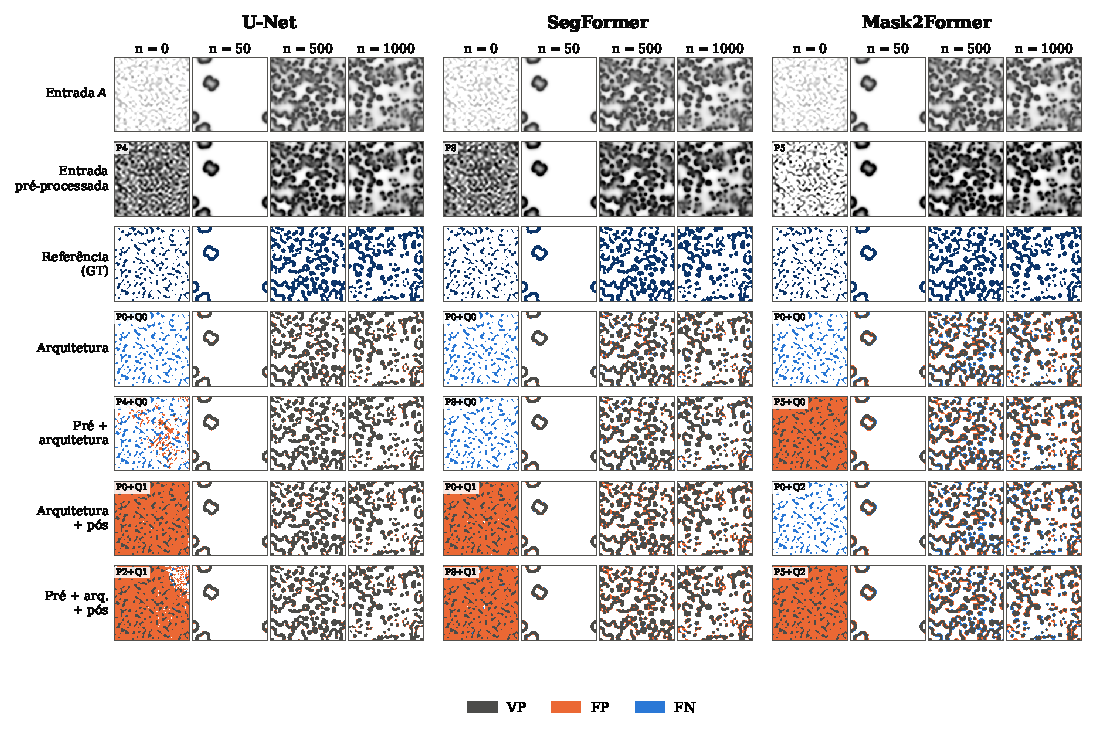
\includegraphics[height=.8\textheight]{visual_table_spirals}
  \end{center}

  \vspace{-1.1em}
  \leg{Cinza: acerto; laranja: falso positivo; azul: falso negativo.
  Instantes 0, 50, 500 e 1000.}

\end{frame}

% -----------------------------------------------------------------------------
\begin{frame}{Efeito de cada técnica}

  \begin{center}
    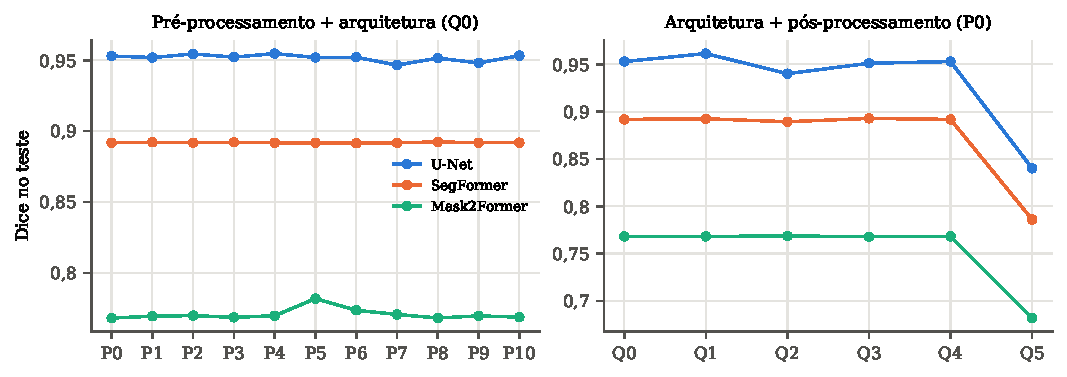
\includegraphics[width=.84\textwidth]{effects_pre_post}
  \end{center}

  \vspace{-.5em}
  \begin{itemize}
    \item Pré-processamento: no máximo 1,37 ponto (recorte por percentis no Mask2Former).
    \item Mediana e difusão anisotrópica pioram a U-Net em 0,64 e 0,49 ponto.
    \item Filtro temporal: perda de 8,6 a 11,3 pontos; cerca de 30 em \textit{gliders} e \textit{spirals}.
  \end{itemize}

\end{frame}

% -----------------------------------------------------------------------------
\begin{frame}{O instante inicial decide a seleção}

  \begin{columns}[T,onlytextwidth]
    \column{.5\textwidth}
      \small
      \begin{tabular}{lccc}
        \toprule
        Dice & todos & $n=0$ & $n\geq50$ \\
        \midrule
        U-Net P0+Q0 & 0,953 & 0,120 & \textbf{0,995} \\
        U-Net P2+Q1 & \textbf{0,962} & 0,354 & 0,992 \\
        \addlinespace
        SegFormer P0+Q0 & 0,892 & 0,100 & \textbf{0,931} \\
        SegFormer P8+Q1 & \textbf{0,893} & 0,357 & 0,920 \\
        \addlinespace
        Otsu em $A$ & 0,888 & 0,241 & 0,921 \\
        \bottomrule
      \end{tabular}
    \column{.46\textwidth}
      Em $n=0$ o campo é aleatório e $A$ ainda não informa $B$.

      Com limiar 0,2 a U-Net marca 95\% do domínio nesse quadro e o Dice dele
      sobe de 0,12 para 0,35.

      Sem $n=0$, a otimização do limiar passa a \alert{piorar} a U-Net
      ($-0,28$) e o SegFormer ($-1,21$).
  \end{columns}

  \vspace{.4em}
  \leg{Um quadro entre 21, sem informação física, foi suficiente para escolher a
  configuração na validação.}

\end{frame}

% -----------------------------------------------------------------------------
\begin{frame}{Evolução temporal}

  \begin{center}
    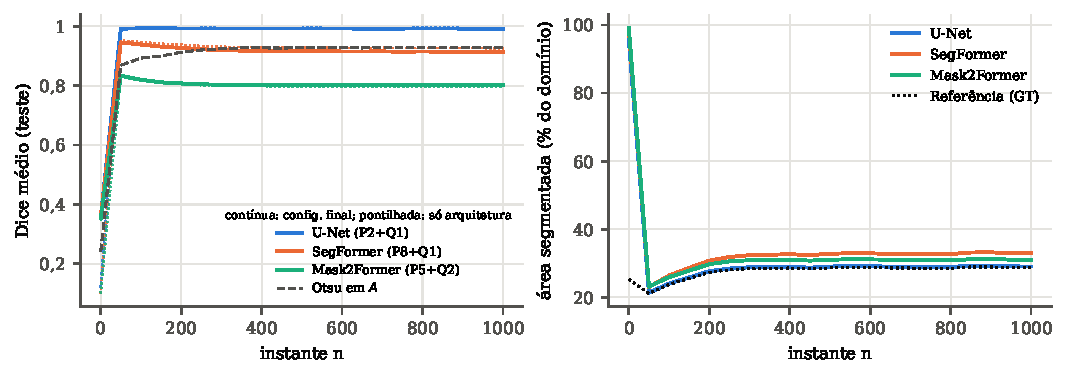
\includegraphics[width=.84\textwidth]{temporal_dice_area}
  \end{center}

  \vspace{-.5em}
  \begin{itemize}
    \item A partir de $n=50$ a U-Net acompanha as estruturas: Dice de 0,995.
    \item Erro de área de 0,76\% do domínio por instante e erro de centroide de 2,7 pixels.
    \item SegFormer e Mask2Former: erro de centroide de 7 a 10 pixels.
  \end{itemize}

\end{frame}

% =============================================================================
\section{Discussão}

% -----------------------------------------------------------------------------
\begin{frame}{Por que melhorou ou piorou}

  \begin{itemize}
    \item \textbf{Resolução de saída.} Com estruturas de 5 a 12 pixels, uma célula de
      $32\times32$ cobre boa parte de uma mancha. O SegFormer cai justamente nos
      regimes de menor comprimento de onda.
    \item \textbf{Dados sem ruído.} Filtros de suavização retiram detalhe que a U-Net
      usava; normalizações afins são absorvidas pela própria rede.
    \item \textbf{Escala da morfologia.} A abertura de raio 1 apaga paredes finas de
      \textit{bubbles}; o filtro de componentes não encontra ruído para remover.
    \item \textbf{Amostragem temporal.} Quadros separados por 500 unidades de tempo:
      a mediana atrasa estruturas que se movem.
  \end{itemize}

  \leg{O desenho não separa resolução de saída de \textit{backbone} e pré-treino.
  Uma semente por treino.}

\end{frame}

% -----------------------------------------------------------------------------
\begin{frame}{Conclusões}

  \begin{itemize}
    \item A U-Net segmentou o Gray-Scott com Dice de 0,953, acima da limiarização
      de $A$ (0,888); SegFormer e Mask2Former não superaram essa referência.
    \item Pré e pós-processamento mudaram pouco o resultado; o filtro temporal
      prejudicou os regimes dinâmicos.
    \item A resolução de saída da arquitetura pesou mais que as técnicas ao redor dela.
    \item Escolher pelo Dice médio favoreceu supersegmentar o quadro inicial.
      Para os outros fluidos da turma vale excluir ou ponderar $n=0$.
  \end{itemize}

  \vspace{.3em}
  \leg{Próximos passos: mais sementes, Mask2Former com supervisão profunda e
  saída em resolução maior nos Transformers.}

\end{frame}

% -----------------------------------------------------------------------------
\begin{frame}{Referências}

  \footnotesize
  \begin{itemize}
    \item[] Gray, P.; Scott, S. K. Autocatalytic reactions in the isothermal,
      continuous stirred tank reactor. \textit{Chem. Eng. Sci.}, 38(1), 1983.
    \item[] Pearson, J. E. Complex patterns in a simple system.
      \textit{Science}, 261(5118), 1993.
    \item[] Ohana, R. et al. The Well: a large-scale collection of diverse physics
      simulations for machine learning. \textit{NeurIPS}, 2024.
    \item[] Ronneberger, O.; Fischer, P.; Brox, T. U-Net. \textit{MICCAI}, 2015.
    \item[] Xie, E. et al. SegFormer. \textit{NeurIPS}, 2021.
    \item[] Cheng, B. et al. Masked-attention mask transformer for universal image
      segmentation. \textit{CVPR}, 2022.
    \item[] Otsu, N. A threshold selection method from gray-level histograms.
      \textit{IEEE Trans. SMC}, 9(1), 1979.
  \end{itemize}

\end{frame}

\end{document}
